\section{Weighted Strichartz estimate for the free Schr\"odinger equation}

In this section we prove a weighted Strichartz estimate from \cite{arxiv:1805.02775}.
That article actually proves a more elaborate estimate using also some results from \cite{MR3842310} as an input, but the more elaborate version does not give better results for fractal weights.

\subsection{Notation}
We will prove a priori estimates for solutions $u = \eit f$ of the free Schr\"odinger equation with initial data $f \in L^{2}(\R^{n})$.
The estimate will be on a ball of spatial scale $R$.
For a small $\delta$ we consider small balls of scale $K^{2}$, where $K=R^{\delta}$ will be the parameter in the Bourgain--Guth argument.
By parabolic rescaling we will get a bunch of tubes of different sizes summarized below.
\begin{center}
\begin{tabular}{cccc} \toprule
  Name & Symbol & Size before scaling & Size after scaling\\ \midrule
  Big & $\bB$ & $R$ & \\
  Small & $\bS$ & $K^{2}$ & \\
  Big at previous scale & $\bBp$ & $R/K \times R$ & $R/K^{2} = R_{1}$\\
  Small at previous scale & $\bSp$ & $KK_{1}^{2} \times K^{2}K_{1}^{2}$ & $K_{1}^{2}$\\ \midrule
  Outer & $\bO$ & $R/r \times R$ & \\
  Inner & $\bI$ & $K^{2} r^{1-4\delta} \times K^{2} r^{2-4\delta}$ & \\
  Outer at previous scale& $\bOp$ & $R/(Kr) \times R$ & $R/(K^{2}r) \times R/K^{2}$\\
  Inner at previous scale & $\bIp$ & $K K_{1}^{2} r^{1-4\delta} \times K^{2} K_{1}^{2} r^{2-4\delta}$ & $K_{1}^{2} r^{1-4\delta} \times K_{1}^{2} r^{2-4\delta}$\\
  \bottomrule
\end{tabular}
\end{center}
The following possible inclusions will be relevant: $\bB \supset \bBp \supset \bSp \supset \bS$ (for the latter inclusion it is important that $\delta \leq 1/4$).


\subsection{Weighted estimate}

\begin{proposition} \label{prop:fractal-strichartz2}
Let $n\geq 1$ and $E,E'$ suitably large depending on $n$.
Let $p=\frac{2(n+1)}{n-1}$ ($p=\infty$ when $n=1$).
Fix $\delta \in (0,1/4)$.

Let $2 \leq t \leq 2(n+1)/n$, $p_{\mathrm{mr},n}=2(n+1)/n$, $p_{\mathrm{dec},n-1}=2(n+1)/(n-1)$,
\[
\frac{1}{t_{1}} = \frac{1}{t} - \frac{1}{p_{\mathrm{mr},n}}, \quad
\frac{1}{t_{2}} = \frac{1}{t} - \frac{1}{p_{\mathrm{dec},n-1}}, \quad
\frac{1}{t_{3}} = \frac{n+2}{p_{\mathrm{dec},n-1}} - \frac{n}{2} = - \frac{1}{n+1}.
\]
For $R\geq 1$ let $\FrStr(R)$ denote the smallest constant such that the following holds with $K=R^{\delta}$.

For every non-negative weight function $(\mu_{\bS})$ and every function $f$ with $\supp \widehat{f}\subset B^n(0,1)$ we have
\begin{equation}\label{eq:fractal-strichartz2}
\ell^{t}_{\bS \subset \bB} \mu_{\bS} \norm{ u }_{L^{p}(w_{\bS,E})}
\leq
\FrStr(R) W R^{-1/2} \norm{ u }_{L^{2}(w_{\bB,E'})}.
\end{equation}
with
\[
W := \sup_{1 \leq r \leq R^{1/2}} r^{1/t_{3}} \sup_{\bO} \ell^{t_{1}}_{\bI \subset \bO} \ell^{t_{2}}_{\bS \subset \bI} \mu_{\bS}.
\]
Then
\[
\FrStr(R) \leq
C_{\epsilon} K^{C_{\epsilon}} R^{\epsilon} + C_{\epsilon'} K^{\epsilon'} \FrStr(R/K^{2}).
\]
\end{proposition}

\begin{corollary}
\label{cor:fractal-strichartz2}
If $\delta$ is sufficiently small depending on $\epsilon$, then
\begin{equation}\label{eq:fractal-strichartz2}
\ell^{t}_{\bS \subset \bB} \mu_{\bS} \norm{ u }_{L^{p}(\bS)}
\lesssim_{\epsilon}
W R^{\epsilon} \norm{ f }_{L^{2}(\R^{n})}.
\end{equation}
\end{corollary}

In the remaining part of this section we prove Proposition~\ref{prop:fractal-strichartz2}.

\paragraph{Bourgain--Guth argument}
Denote by $\Part{K^{-1}}$ the set of $K^{-1}$-cubes inside the unit ball in the frequency space $\R^{n}$.
Using a smooth partition of unity we decompose $f = \sum_{\tau \in \Part{K^{-1}}} f_{\tau}$ and $u_{\tau} = \eit f_{\tau}$ accordingly.
Given a $K^2$-cube $\bS \subset \R^{n+1}$, we define its \emph{significant} set
\[
\calS(\bS):=\Set[\Big]{\tau \in \Part{K^{-1}} \given \norm{u_\tau}_{L^p(w_{\bS,E})} \geq \frac{\norm{u}_{L^p(w_{\bS,E})}}{100(\#\Part{K^{-1}})} }.
\]
We say a $K^2$-cube $\bS$ is \emph{narrow} if there is an $(n-1)$-dimensional subspace $V \subset \R^{n}$ such that all cubes in $\calS(\bS)$ are $100/K$-close to $V$, and \emph{broad} otherwise.
Then for any broad cube $\bS$ there exist $\nu$-transverse cubes $\tau_1,\dotsc, \tau_{n+1} \in \calS(\bS)$ with $\nu \gtrsim K^{-n}$.

\paragraph{Localized multilinear restriction}
Let $\tau_{1},\dotsc,\tau_{n+1} \in \Part{K^{-1}}$ be $\nu$-transverse.
Then from multilinear restriction we can deduce
\[
\ell^{2(n+1)/n}_{\bS \subset \bB} \avprod \norm{ \tilde{u}_{\tau_{j}} }_{L^{p}(\bS)}
\lesssim_{\epsilon}
K^{C} \nu^{-C_{\epsilon}} R^{-1/2+\epsilon} \avprod \norm{ \tilde{u}_{\tau_{j}} }_{L^{2}(\R^{n+1})}
\]
for any functions $\tilde{u}_{\tau}$ supported in the $R^{-1}$-neighborhood of the paraboloid over $\tau$.
In particular this holds for $\tilde{u}_{\tau} = u_{\tau} \psi_{\bB}$ for some bump function of scale $R$ adapted to the ball $\bB$ whose Fourier transform is supported in an $R^{-1}$-neighborhood of $0$, and it follows that
\begin{align*}
\ell^{2(n+1)/n}_{\bS \subset \bB} \avprod \norm{ u_{\tau_{j}} }_{L^{p}(\bS)}
&\lesssim_{\epsilon,E''}
K^{C} \nu^{-C_{\epsilon}} R^{-1/2+\epsilon} \avprod \norm{ u_{\tau_{j}} }_{L^{2}(w_{\bB,E''})}\\
&\lesssim_{E'',E'''}
K^{C} \nu^{-C_{\epsilon}} R^{-1/2+\epsilon} \norm{ u }_{L^{2}(w_{\bB,E'''})},
\end{align*}
where we use that $u_{\tau}$ is a convolution of $u$ with an $L^{1}$ normalized smooth kernel.
By an averaging procedure similar to that in the proof of decoupling this implies
\begin{equation}
\label{eq:mult-restr:local}
\ell^{2(n+1)/n}_{\bS \subset \bB} \avprod \norm{ u_{\tau_{j}} }_{L^{p}(w_{\bS,E})}
\lesssim_{\epsilon,E,E'}
K^{C} \nu^{-C_{\epsilon}} R^{-1/2+\epsilon} \norm{ u }_{L^{2}(w_{\bB,E'})}
\end{equation}
for some suitable $E,E'$.

\paragraph{Broad case}
If $\bS$ is broad, then for some $\nu$-transverse $\tau_{1},\dotsc,\tau_{n+1} \in \Part{K^{-1}}$ depending on $\bS$ we have
\[
\norm{ u }_{L^{p}(w_{\bS,E})}
\lesssim
K^{C} \avprod_{j=1}^{n+1} \norm{ u_{\tau_{j}} }_{L^{p}(w_{\bS,E})}
\]
so for the sum over broad $\bS$ by \eqref{eq:mult-restr:local} we have
\begin{align*}
\ell^{t}_{\bS \subset \bB} \mu_{\bS} \norm{ u }_{L^{p}(w_{\bS,E})}
&\lesssim
K^{C} \ell^{t}_{\bS \subset \bB} \mu_{\bS}
\sup_{\substack{\tau_{1},\dotsc,\tau_{n+1}\in\Part{K^{-1}}\\ \nu-\text{transverse}}}
\avprod \norm{ u_{\tau_{j}} }_{L^{p}(w_{\bS,E})}\\
&\leq
K^{C} W_{\bB} \ell^{2(n+1)/n}_{\bS \subset \bB}
\sup_{\substack{\tau_{1},\dotsc,\tau_{n+1}\in\Part{K^{-1}}\\ \nu-\text{transverse}}}
\avprod \norm{ u_{\tau_{j}} }_{L^{p}(w_{\bS,E})}\\
&\leq
K^{C} W_{\bB}
\sum_{\substack{\tau_{1},\dotsc,\tau_{n+1}\in\Part{K^{-1}}\\ \nu-\text{transverse}}}
\ell^{2(n+1)/n}_{\bS \subset \bB} \avprod \norm{ u_{\tau_{j}} }_{L^{p}(w_{\bS,E})}\\
&\lesssim_{\epsilon}
\nu^{-C_{\epsilon}} K^{C} R^{\epsilon} W_{\bB}
\sum_{\substack{\tau_{1},\dotsc,\tau_{n+1}\in\Part{K^{-1}}\\ \nu-\text{transverse}}}
R^{-1/2} \norm{u}_{L^{2}(w_{\bB,E'})}\\
&\lesssim
K^{C_{\epsilon}} R^{\epsilon}
W_{\bB} R^{-1/2} \norm{u}_{L^{2}(w_{\bB,E'})},
\end{align*}
where $W_{\bB} = \ell^{t_{1}}_{\bS \subset \bB} \mu_{\bS} \leq W$.
This finishes the estimate for the contribution of the broad cubes.

\paragraph{Narrow case}
If the cube $\bS$ is narrow, then by lower-dimensional decoupling we have
\begin{align*}
\norm{u}_{L^p(w_{\bS,E})}
&\sim
\norm[\big]{\sum_{\tau\in \calS(\bS)}u_\tau}_{L^p(w_{\bS,E})}\\
&\lesssim_{\epsilon} K^{\epsilon}
\ell^{2}_{\tau\in \calS(\bS)} \norm{u_\tau}_{L^p(w_{\bS,E})}\\
&\leq K^{\epsilon}
\ell^{2}_{\tau} \norm{u_\tau}_{L^p(w_{\bS,E})}.
\end{align*}
Summing over narrow $\bS$ it remains to estimate
\begin{align*}
\ell^{t}_{\bS \subset \bB} \ell^{2}_{\tau} \mu_{\bS} \norm{ u_{\tau} }_{L^{p}(w_{\bS,E})}
&\leq
\ell^{2}_{\tau} \ell^{t}_{\bS \subset \bB} \mu_{\bS} \norm{ u_{\tau} }_{L^{p}(w_{\bS,E})}\\
&\lesssim
\ell^{2}_{\tau} \ell^{t}_{\bBp : \tau} \ell^{t}_{\bS \subset \bBp} \mu_{\bS} \norm{ u_{\tau} }_{L^{p}(w_{\bS,E})}\\
&\lesssim
\ell^{2}_{\tau} \ell^{2}_{\bBp : \tau} \ell^{t}_{\bS \subset \bBp} \mu_{\bS} \norm{ u_{\tau} }_{L^{p}(w_{\bS,E})},
\end{align*}
where for each $\tau$ we sum over tubes $\bBp$ polar to $\tau$.
Fixing $\tau$ and $\bBp$ polar to $\tau$ we obtain
\begin{equation} \label{eq:fixed-Box-norm2}
\begin{split}
\ell^{t}_{\bS \subset \bBp} \mu_{\bS} \norm{ u_{\tau} }_{L^{p}(w_{\bS,E})}
&\lesssim
\ell^{t}_{\bSp \subset \bBp} \ell^{t}_{\bS \subset \bSp} \mu_{\bS} \norm{ u_{\tau} }_{L^{p}(w_{\bS,E})}\\
&\leq
\ell^{t}_{\bSp \subset \bBp} \mu_{\bSp} \ell^{p}_{\bS \subset \bSp} \norm{ u_{\tau} }_{L^{p}(w_{\bS,E})}\\
&\lesssim
\ell^{t}_{\bSp \subset \bBp} \mu_{\bSp} \norm{ u_{\tau} }_{L^{p}(w_{\bSp,E})},
\end{split}
\end{equation}
where
\[
\mu_{\bSp} := \ell^{t_{2}}_{\bS \subset \bSp} \mu_{\bS}.
\]
Recall parabolic scaling $L_{\tau}$ and scaling/modulation operators $M_{\tau}$ that we used in the proof of the decoupling inequality.
\begin{center}
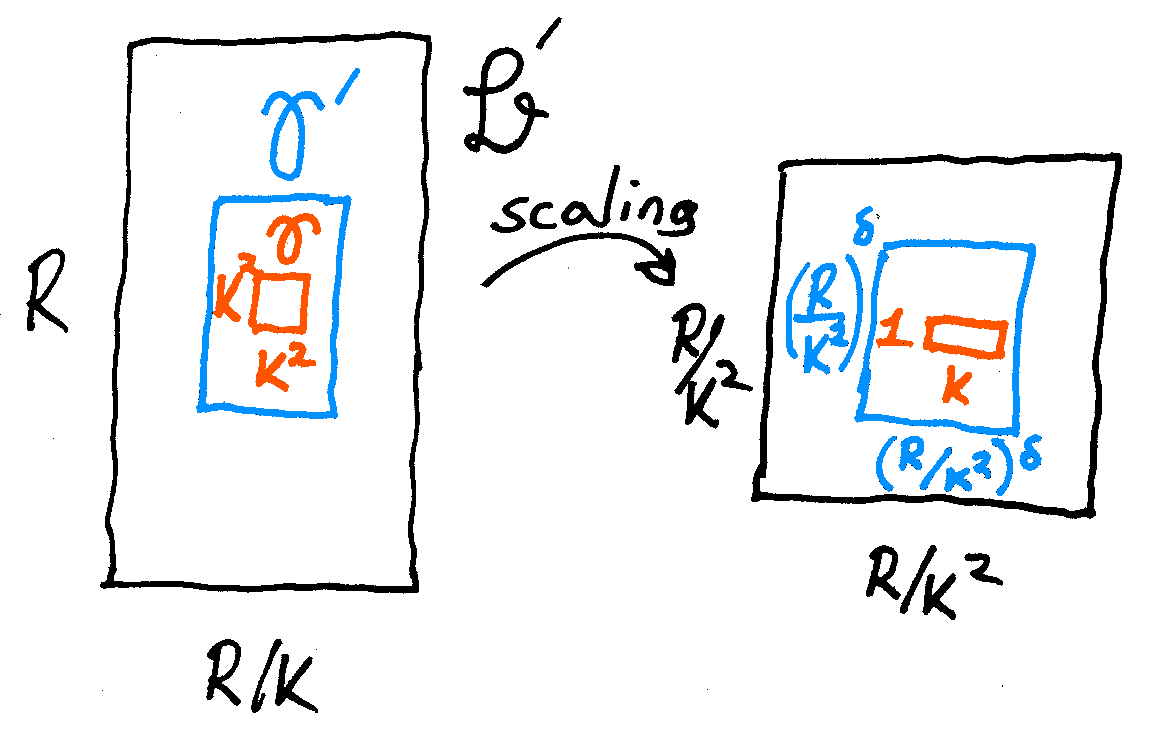
\includegraphics[height=4cm]{max-schroedinger-scaling.png}
\end{center}
We have
\begin{align*}
\eqref{eq:fixed-Box-norm2}
%\ell^{t}_{\bSp \subset \bBp} \mu_{\bSp} \norm{ u_{\tau} }_{L^{p}(w_{\bSp,E})}
&=
K^{(n+2)/p} \ell^{t}_{\bSp \subset \bBp} \mu_{\bSp} \norm{ M_{\tau}^{-1} u_{\tau} }_{L^{p}(w_{L_{\tau}\bSp,E})}\\
&\leq
K^{(n+2)/p} \FrStr(R/K^{2}) W' (R/K^{2})^{-1/2} \norm{ M_{\tau}^{-1} u_{\tau} }_{L^{2}(w_{L_{\tau}\bBp,E'})}\\
&=
K^{(n+2)/p} \FrStr(R/K^{2}) W' (R/K^{2})^{-1/2} K^{-(n+2)/2} \norm{ u_{\tau} }_{L^{2}(w_{\bBp,E'})}\\
&=
K^{-1/(n+1)} \FrStr(R/K^{2}) W' R^{-1/2} \norm{ u_{\tau} }_{L^{2}(w_{\bBp,E'})}
\end{align*}
where $W'$ is computed using the new weights $\mu_{\bSp}$.
Since
\[
\ell^{2}_{\tau} \ell^{2}_{\bBp : \tau} \norm{u_{\tau}}_{L^{2}(w_{\bBp,E'})}
\lesssim
\ell^{2}_{\tau} \norm{u_{\tau}}_{L^{2}(w_{\bB,E'})}
\lesssim
\norm{u}_{L^{2}(w_{\bB,E'})},
\]
where we used a localized square function estimate, it remains to observe
\begin{equation}
\label{eq:big-const2}
K^{-1/(n+1)} W'
\lesssim
W.
\end{equation}
Indeed, every $r$ in the definition of $W'$ corresponds to $Kr$ in the definition of $W$.
This finishes the estimate for the narrow cubes and completes the proof of Proposition~\ref{prop:fractal-strichartz2}.

\subsection{Consequences for fractal measures}
Now we evaluate $W$ in the case when $(\mu_{\bS})$ is the characteristic function of an $\alpha$-dimensional set.
Specifically, we assume that $\mu_{\bS} \in \Set{0,1}$ and for any $K^{2} \leq r \leq R$ and $x$ we have
\begin{equation}
\label{eq:mu-alpha-dim}
\sum_{\bS \subseteq B(x,r)} \mu_{\bS} \lesssim r^{\alpha}.
\end{equation}
Note that $t_{2} < t_{1}$, and it follows that
\begin{multline*}
W
=
\sup_{1 \leq r \leq R^{1/2}} r^{-1/(n+1)} \sup_{\bO} \Bigl( \sum_{\bI \subset \bO} \bigl( \sum_{\bS \subset \bI} \mu_{\bS}^{t_{2}} \bigr)^{t_{1}/t_{2}}  \Bigr)^{1/t_{1}}\\
\leq
\sup_{1 \leq r \leq R^{1/2}} r^{-1/(n+1)} \sup_{\bO} \Bigl( \sum_{\bI \subset \bO} \bigl( \sum_{\bS \subset \bI} \mu_{\bS}^{t_{2}} \bigr) \cdot \sup_{\bI \subset \bO} \bigl( \sum_{\bS \subset \bI} \mu_{\bS}^{t_{2}} \bigr)^{t_{1}/t_{2}-1}  \Bigr)^{1/t_{1}}\\
\leq
\sup_{1 \leq r \leq R^{1/2}} r^{-1/(n+1)} \sup_{\bO} \Bigl( \sum_{\bS \subset \bO} \mu_{\bS}^{t_{2}} \Bigr)^{1/t_{1}} \cdot \sup_{\bI \subset \bO} \bigl( \sum_{\bS \subset \bI} \mu_{\bS}^{t_{2}} \bigr)^{1/t_{2}-1/t_{1}}
\end{multline*}
Under the hypothesis \eqref{eq:mu-alpha-dim} with $\alpha\geq 1$ this is
\begin{multline*}
\lessapprox
\sup_{1 \leq r \leq R^{1/2}} r^{1/t_{3}} \Bigl( r (R/r)^{\alpha} \Bigr)^{1/t_{1}} \cdot \bigl( r r^{\alpha} \bigr)^{1/t_{2}-1/t_{1}}\\
=
R^{\alpha/t_{1}} \sup_{1 \leq r \leq R^{1/2}} r^{1/t_{2}+1/t_{3}} r^{\alpha(1/t_{2}-2/t_{1})}
=
R^{\alpha/t_{1}} \sup_{1 \leq r \leq R^{1/2}} r^{1/t-1/2} r^{\alpha(1/2-1/t)}\\
=
R^{\alpha/t_{1}} \sup_{1 \leq r \leq R^{1/2}} r^{(\alpha-1)(1/2-1/t)}
=
R^{\alpha/t_{1}} R^{(\alpha-1)(1/2-1/t)/2},
\end{multline*}
assuming $\alpha \geq 1$.
By Corollary~\ref{cor:fractal-strichartz2} with $t=2$ and the above estimate we obtain
\begin{equation}
\label{eq:max-frac-Schroedinger}
\boxed{\ell^{2}_{\bS \subset \bB} \mu_{\bS} \norm{ u }_{L^{p}(\bS)}
\lessapprox
R^{\alpha/(2(n+1))} \norm{f}_{2}.}
\end{equation}
Up to some uncertainty principle considerations this is the sharp $L^{2}$ estimate for the Schr\"odinger maximal function on sets of dimension $\alpha$ proved in \cite[Theorem 2.2]{arxiv:1805.02775}.

With $\alpha=n=1$ and $t=4$ one can also recover, up to the endpoint, the $L^{4}(\R)$ estimate for the Schr\"odinger maximal function \cite{MR1101221}.

One can rescale estimates on a ball of radius $R$ for functions with Fourier support in the unit ball to estimates on a ball of radius $1$ for functions with Fourier support in a ball of radius $R$.
Summing these estimates one can formulate these estimates also on $H^{s}$ spaces, see \cite{MR2264734}.

\subsection{Lower bounds}
Applying \eqref{eq:max-frac-Schroedinger} with $\alpha=n$ and using parabolic scaling we see that
\begin{equation}
\label{eq:max-Lebesgue-Schroedinger}
\norm{ \sup_{0 < t < 1/R} \abs{e^{it\Delta} f} }_{L^{2}(B^{n}(0,1))}
\lessapprox R^{\frac{n}{2(n+1)}} \norm{f}_{L^{2}(\R^{n})}
\end{equation}
for any function $f$ with $\supp \widehat{f} \subset B(0,R)$.
In this section we will show that this $L^{2}$ bound for the Schr\"odinger maximal function is optimal up to the $R^{\epsilon}$ loss.
To this end we use special solutions considered in \cite{MR2354692} and \cite{MR3613507}.
The lower bound that we will show was first proved in \cite{MR3574661}, but we follow the argument in \cite{arxiv:1703.01360}.
Lower bounds for $L^{2}\to L^{p}$ estimates using the same construction were obtained in \cite{arxiv:1902.01430}.

\subsubsection{Modulation of initial data}
Suppose that $u = e^{it\Delta} f$, or more precisely
\[
u(x,t) = \int \widehat{f}(\xi) e(x\xi + t \abs{\xi}^{2}) \dif\xi.
\]
Modulate $f$ by a frequency $\eta$, so that $f_{\eta}(x) = f(x) e(x\eta)$, and let $u_{\eta} = e^{it\Delta} f_{\eta}$, so that
\begin{align*}
u_{\eta}(x,t)
&=
\int \widehat{f}(\xi-\eta) e(x\xi + t \abs{\xi}^{2}) \dif\xi
\\ &=
\int \widehat{f}(\xi) e(x\xi+x\eta + t \abs{\xi+\eta}^{2}) \dif\xi
\\ &=
e(x\eta + t\abs{\eta}^{2})\int \widehat{f}(\xi) e(x\xi + t \abs{\xi}^{2} + 2 t \xi\eta) \dif\xi
\\ &=
e(x\eta + t\abs{\eta}^{2}) u(x+2t\eta,t).
\end{align*}
So we see that a modulation of the initial data by $\eta$ causes the solution to travel with speed $-2\eta$.
We will construct a solution that is large on some set for many times $t$, and then shift it around using this observation.

\subsubsection{Many wave packets}
We work in dimension $1$.
Fix $0<\sigma<1$.
Let $f$ be given by
\[
\widehat{f_{\mathrm{many}}}(\xi)
=
\widehat{f}(\xi)
=
\sum_{\abs{l} \leq 2R^{\sigma}} \phi(\xi-R^{1-\sigma}l),
\]
where $\phi$ is a smooth positive function with $\phi(0)=1$ supported on a small $\rho$-neighborhood of the origin.
Then
\begin{align*}
e^{i(t/R)\Delta} f(x)
&=
\int \widehat{f}(\xi) e(x \xi + (t/R) \abs{\xi}^{2}) \dif\xi
\\ &=
\sum_{\abs{l} \leq 2R^{\sigma}} \int \phi(\xi-R^{1-\sigma}l) e(x \xi + (t/R) \abs{\xi}^{2}) \dif\xi
\\ &=
\sum_{\abs{l} \leq 2R^{\sigma}} \int \phi(\xi) e(x (\xi+R^{1-\sigma}l) + (t/R) \abs{\xi+R^{1-\sigma}l}^{2}) \dif\xi
\end{align*}
Assume $x=x_{0}+\tilde{x}$ with $x_{0}\in R^{\sigma-1}\Z$, $\abs{x_{0}} \leq 2$, and $\abs{\tilde{x}} \leq R^{-1}/100$.
Assume $t \in R^{2\sigma-1}\Z$ and $\abs{t} \leq 1$.
Then
\begin{align*}
e^{i(t/R)\Delta} f(x)
&=
\sum_{\abs{l} \leq 2R^{\sigma}} \int \phi(\xi) e((x_{0}+\tilde{x}) (\xi+R^{1-\sigma}l) + (t/R) \abs{\xi+R^{1-\sigma}l}^{2}) \dif\xi
\\ &=
\sum_{\abs{l} \leq 2R^{\sigma}} \int \phi(\xi) e(x_{0}\xi + \tilde{x}(\xi+R^{1-\sigma}l) + (t/R) \abs{\xi}^{2} + (t/R) 2\xi R^{1-\sigma}l) \dif\xi
\\ &\sim
R^{\sigma}
\end{align*}
since the phase is small.

\subsubsection{One wave packet}
We still work in dimension $1$.
Let $f$ be given by
\[
\widehat{f_{\mathrm{one}}}(\xi)
=
\widehat{f}(\xi)
=
\phi(R^{-1/2}\xi).
\]
Then, assuming $\abs{x} \leq R^{-1/2}$ and $\abs{t} \leq 1$, we obtain
\[
e^{i (t/R) \Delta} f
=
\int \widehat{f}(\xi) e(x \xi + (t/R) \abs{\xi}^{2}) \dif\xi
\sim
R^{1/2}
\]
since the phase is small.

\subsubsection{Tensor products}
If $u_{j} = e^{it\Delta} f_{j}$, then
\[
u_{1}(x_{1},t) \dotsm u_{n}(x_{n},t)
=
e^{it\Delta} (f_{1}\otimes\dotsm\otimes f_{n})(x_{1},\dotsc,x_{n}).
\]
We combine the previous examples by taking a tensor product:
\[
f = f_{\mathrm{one}} \otimes f_{\mathrm{many}} \otimes \dotsm \otimes f_{\mathrm{many}}.
\]
Then the solution $u = e^{i(t/R)\Delta} f$ is $\sim R^{1/2 + (n-1)\sigma}$ on the set
\begin{equation}
\label{eq:supp-u}
(-R^{1/2},R^{1/2}) \times \Bigl( \bigl( R^{\sigma-1}\Z \cap (-2,2) \bigr) + (-R^{-1}/100,R^{-1}/100) \Bigr)^{n-1} \times \Bigl( R^{2\sigma-1}\Z \cap (0,1) \Bigr).
\end{equation}
We modulate $f$ by the frequency $\eta = -\frac12 (R, R^{-2\sigma}, R^{-3\sigma},\dotsc, R^{-n\sigma})$.
The absolute value of the new solution is then given by $\abs{u(x+2\eta t, t)}$.
We subdivide time into intervals of length $R^{-1/2}$.
The shifts of \eqref{eq:supp-u} by times from non-adjacent time intervals are then essentially disjoint in the first coordinate.
The other coordinates of $\eta$ are chosen in such a way that increasing the time by $R^{2\sigma-1}$ moves the $2$nd coordinate by $R^{-1}$.
After $R^{\sigma}$ time steps the $2$nd coordinate is shifted by $R^{\sigma-1}$, and the $3$rd coordinate by $R^{-1}$.
After $R^{(n-1)\sigma}$ time steps the shifts of $R^{-1}/100$-cubes then cover a positive proportion of the fundamental domain modulo $R^{\sigma-1}$ in coordinates $x_{2},\dotsc,x_{n}$.
\begin{center}
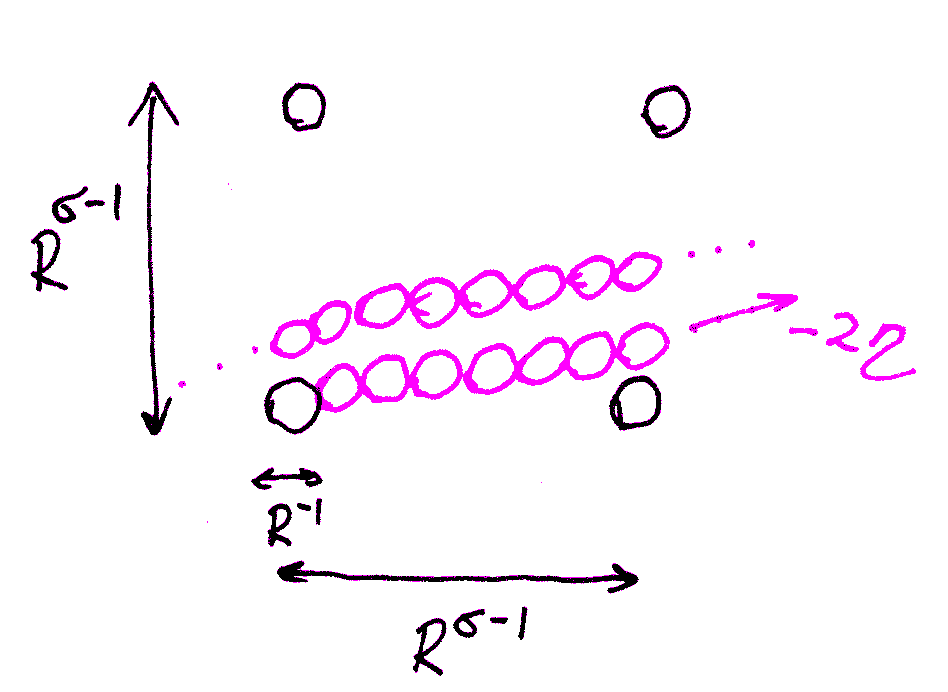
\includegraphics[height=3cm]{luca-rogers-example.png}
\end{center}
Choosing $\sigma=\frac{1}{2(n+1)}$ we see that $R^{(n-1)\sigma}$ time steps of length $R^{2\sigma-1}$ add up to a time interval of length $R^{-1/2}$.
Moreover, the total shift over the time interval $(0,1)$ in coordinates $x_{2},\dotsc,x_{n}$ is bounded by $R^{-2\sigma} \ll 1$.
Hence the new solution is $\sim R^{1/2 + (n-1)\sigma}$ on a set of measure $\sim 1$.
Also, $\norm{f}_{2} \sim R^{(1/2+(n-1)\sigma)/2} \sim R^{n/(2(n+1))}$.
Hence if \eqref{eq:max-Lebesgue-Schroedinger} holds with exponent $s$ in place of $\frac{n}{2(n+1)}$ we obtain
\[
R^{1/2 + (n-1)\sigma} \lesssim R^{s} R^{n/(2(n+1))},
\]
so
\[
s \geq n/(2(n+1)).
\]
\begin{remark}
In \cite{arxiv:1902.01430} the same kind of example with
\[
f = f_{\mathrm{one}}^{\otimes (n-m+1)} \otimes f_{\mathrm{many}}^{\otimes (m-1)},
\quad 1 \leq m \leq n,
\]
is used.
\end{remark}
